\documentclass[conference]{IEEEtran}
\IEEEoverridecommandlockouts
\usepackage{cite}
\usepackage{amsmath,amssymb,amsfonts}
\usepackage{algorithmic}
\usepackage{graphicx}
\usepackage{textcomp}
\usepackage{xcolor}
\usepackage{booktabs}
\usepackage{multirow}
\usepackage{hyperref}
\usepackage{enumitem}
\usepackage{tikz}
\usetikzlibrary{shapes.geometric, arrows, arrows.meta, positioning, calc}

\newcommand{\rev}[1]{\textcolor{blue}{#1}}

% When compiling locally: figures are searched in ../results/ and ../experiments/ablation/figures/
% When uploading to Overleaf: copy all referenced .png files into the same folder as main.tex
\graphicspath{{../results/}{../experiments/ablation/figures/}{../results/tier5_bica_s42/figures/}}

\def\BibTeX{{\rm B\kern-.05em{\sc i\kern-.025em b}\kern-.08em
    T\kern-.1667em\lower.7ex\hbox{X}}}

\begin{document}

\title{Hierarchical Multi-Stream Learning for Eye Movement-Based Schizophrenia Recognition: From Handcrafted Features to Bidirectional Graph--Transformer Ensembles}

\author{Ha-Hai-Van Le$^{1}$, Minh-Tuyen Pham$^{1}$, Hoang-Giang Bui$^{1}$,
        Supervisor: Thanh-Hai Tran$^{1}$, Hanh-Trang Bui$^{1}$\\
$^{1}$School of Electrical and Electronic Engineering\\
Hanoi University of Science and Technology, Hanoi, Vietnam\\
Email: van.lhh233886@sis.hust.edu.vn}

\maketitle

\begin{abstract}
\rev{Schizophrenia recognition from free-viewing eye movements lacks integration between clinical biomarkers and sequence learning. We propose a Hierarchical 5-Tier Framework evaluated on the EMS dataset (208 subjects, EyeLink 1000 Plus 1000\,Hz). The pipeline scales from preprocessing (Tier~1) and feature engineering of stimulus-level and category-wise contrastive delta features (Tier~2) to tabular baselines (Tier~3), parallel deep sequential architectures (Tier~4), and meta-learner ensembling (Tier~5). In Tier~4 we develop two architectures: GNN-CEFAM, a Graph Attention Network with ResNet50-enriched node features ($\mathbb{R}^{69}$) and a Cross-Attention Enhanced Fusion Module; and BiCA-HS, a 4-layer Transformer encoder fused with a 135-dimensional clinical expert stream via bidirectional cross-attention. Both architectures exceed the published performance of the state-of-the-art MSNet baseline (reported test AUC\,=\,0.8854). BiCA-HS achieves an out-of-fold AUC of $0.9549 \pm 0.0039$ (mean $\pm$ std, 3 seeds), and the Tier~5 logistic regression meta-learner reaches AUC\,=\,$0.9590 \pm 0.0009$, improving clinical sensitivity to $88.8 \pm 3.1\%$.}
\end{abstract}

\begin{IEEEkeywords}
schizophrenia, eye movement, scanpath, graph attention network, transformer, cross-attention, ensemble learning, clinical biomarkers.
\end{IEEEkeywords}

\section{Introduction}
\label{sec:introduction}

Schizophrenia is a severe neuropsychiatric disorder affecting approximately 1\% of the global population, characterized by deficits in cognitive control, social cognition, and visual attention \cite{holzman1973}. Clinical diagnosis remains largely qualitative and subject to inter-rater variability, motivating the search for objective, quantifiable biomarkers. Atypical eye movement patterns during free-viewing paradigms have emerged as one of the most replicated neurobiological markers of schizophrenia \cite{benson2012}: patients exhibit restricted visual exploration, social gaze avoidance, and abnormal saccadic dynamics compared to healthy controls \cite{morita2020}.

Existing approaches to eye movement-based schizophrenia classification fall into two broad categories. Hand-crafted feature methods \cite{shpigelman2008, huang2020, tseng2013} extract static summary statistics over fixation sequences and classify them with shallow models, discarding the spatiotemporal structure of scanpaths. Recent deep learning methods such as MSNet \cite{song2025} achieve state-of-the-art performance by aggregating fixation density maps into multi-scale CNN representations; however, this collapses the temporal saccade trajectory and yields no fixation-level clinical interpretability.

To address these limitations, we propose a \textbf{Hierarchical 5-Tier Framework} that systematically integrates clinical domain knowledge with deep representation learning. Our contributions are threefold: 
(1) we introduce Tier 2 contextual delta features (60 cross-category contrast features) that encode stimulus-specific visual response differences clinically linked to social cognition deficits; 
(2) we develop GNN-CEFAM, a spatiotemporal Graph Attention Network featuring a Cross-Attention Enhanced Fusion Module (CEFAM) that computes genuine, non-degenerate cross-attention over pre-pooling fixation nodes; and 
(3) we propose BiCA-HS, a Transformer-based hybrid stream model that fuses raw fixation trajectories with a 135-dimensional clinical expert vector in a unified attention space. Evaluated across three random seeds, our Tier 5 logistic regression meta-learner achieves a state-of-the-art out-of-fold AUC of $0.9590 \pm 0.0009$, achieving higher diagnostic performance than the published MSNet test benchmark (reported AUC\,=\,0.8854).

\section{Related Work}
\label{sec:related_work}

\subsection{Clinical Eye Movement Biomarkers}
Abnormal eye movements under free-viewing conditions are among the most replicated findings in biological psychiatry, reflecting underlying frontal-striatal-cerebellar cognitive dysfunctions \cite{holzman1973}. Benson et al.\ \cite{benson2012} demonstrated that simple free-viewing tests can classify schizophrenia with high accuracy using restricted exploration metrics, while Morita et al.\ \cite{morita2020} reviewed the pathophysiology linking saccadic hypometria and reduced scanpath complexity to psychotic symptom severity.

\subsection{Handcrafted Feature Methods}
Early machine learning classifiers applied SVMs or random forests on static, aggregated eye-tracking metrics such as fixation count, saccade amplitude, and center-bias \cite{shpigelman2008}. Tseng et al.\ \cite{tseng2013} showed that high-throughput classification across multiple clinical populations is achievable from natural viewing. Huang et al.\ \cite{huang2020} introduced discriminative eye movement features combining duration statistics with model-metric descriptors. However, these approaches collapse the spatiotemporal structure of scanpaths and discard sequential dependencies.

\subsection{Deep Scanpath Models}
To capture spatial structures and temporal sequences, deep learning methods have been explored. Recurrent neural networks process raw trajectories but fail to represent non-Euclidean spatial relationships \cite{kasprowski2020}. Song et al.\ \cite{song2025} proposed MSNet on the EMS dataset, using multi-scale CNNs applied to gaze density maps, achieving the current state-of-the-art AUC\,=\,0.8854; however, density-map representations lose temporal ordering and individual fixation interpretability. In parallel, scanpaths have been modeled as spatiotemporal graphs processed by Graph Attention Networks (GAT) \cite{velickovic2018, birawo2024} and as sequence trajectories processed by Transformers \cite{vaswani2017}. Gradient-boosted tree ensembles such as XGBoost \cite{chen2016xgboost}, LightGBM \cite{ke2017lightgbm}, and CatBoost \cite{prokhorenkova2018catboost} offer strong tabular baselines when combined with rich feature engineering.

\subsection{Cross-Attention Fusion}
Fusing heterogeneous feature streams via cross-attention has shown promise in multimodal learning. Naive implementations that unsqueeze both streams to sequence length 1 produce degenerate softmax distributions (value $\equiv$ 1.0) that provide no learning signal. Our CEFAM addresses this by performing genuine cross-attention between the expert embedding and the \textit{pre-pooling} fixation node sequence $H_\text{nodes} \in \mathbb{R}^{N \times 256}$.

\section{Preprocessing and Feature Engineering}
\label{sec:features}

\subsection{Tier 1: Preprocessing}
Raw eye-tracking recordings contain blinks, boundary violations, and micro-saccade oscillations. We apply two sequential filters. \textbf{(1) Spatial filter:} fixations outside the $1024{\times}768$ stimulus screen are discarded ($5{,}037$ of $293{,}740$ raw fixations removed; $1.71\%$). \textbf{(2) Temporal filter:} fixations shorter than 50\,ms are removed as post-saccadic tremor artifacts ($7{,}666$ removed; $2.66\%$), \rev{yielding $281{,}037$ clean fixations across 16,716 total trials. This results in an average of $16.81 \pm 7.73$ fixations per subject per stimulus image (median: 15, max: 44, with $75\%$ of trials containing 20 or fewer fixations), while preserving the pupil size metrics (\texttt{FIX\_PUPIL}). Fig.~\ref{fig:tier1_filtering} visualizes these filtering steps on a sample scanpath.}

\begin{figure}[htbp]
\centering
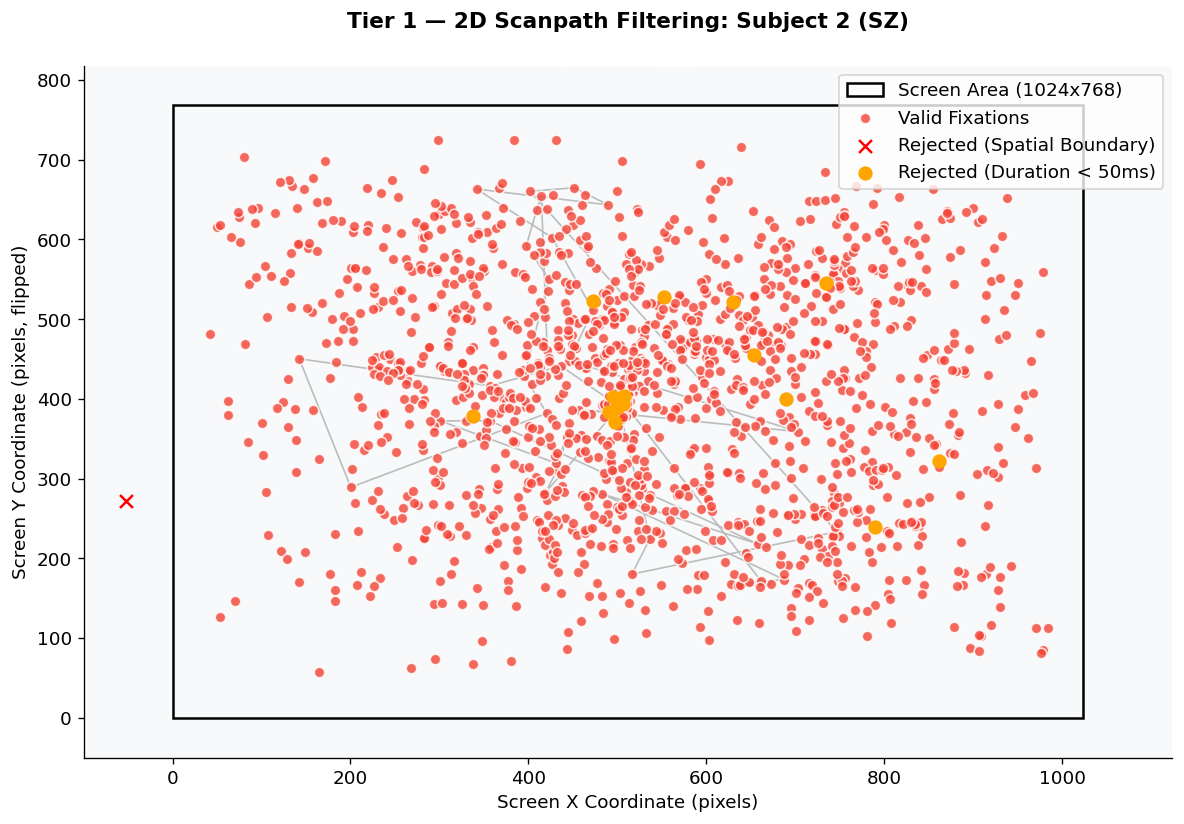
\includegraphics[width=0.95\columnwidth]{tier1_2d_filtering.png}
\vspace{-2mm}
\caption{\rev{Tier 1 scanpath preprocessing visualization for a sample subject. The black rectangle defines the stimulus screen boundaries ($1024\times768$). Red circles represent valid fixations, while red crosses represent fixations rejected due to boundary violations (spatial filtering), and orange circles indicate fixations shorter than 50\,ms rejected as post-saccadic tremor artifacts (temporal filtering).}}
\vspace{-3mm}
\label{fig:tier1_filtering}
\end{figure}

\begin{figure*}[t]
\centering
\resizebox{\textwidth}{!}{%
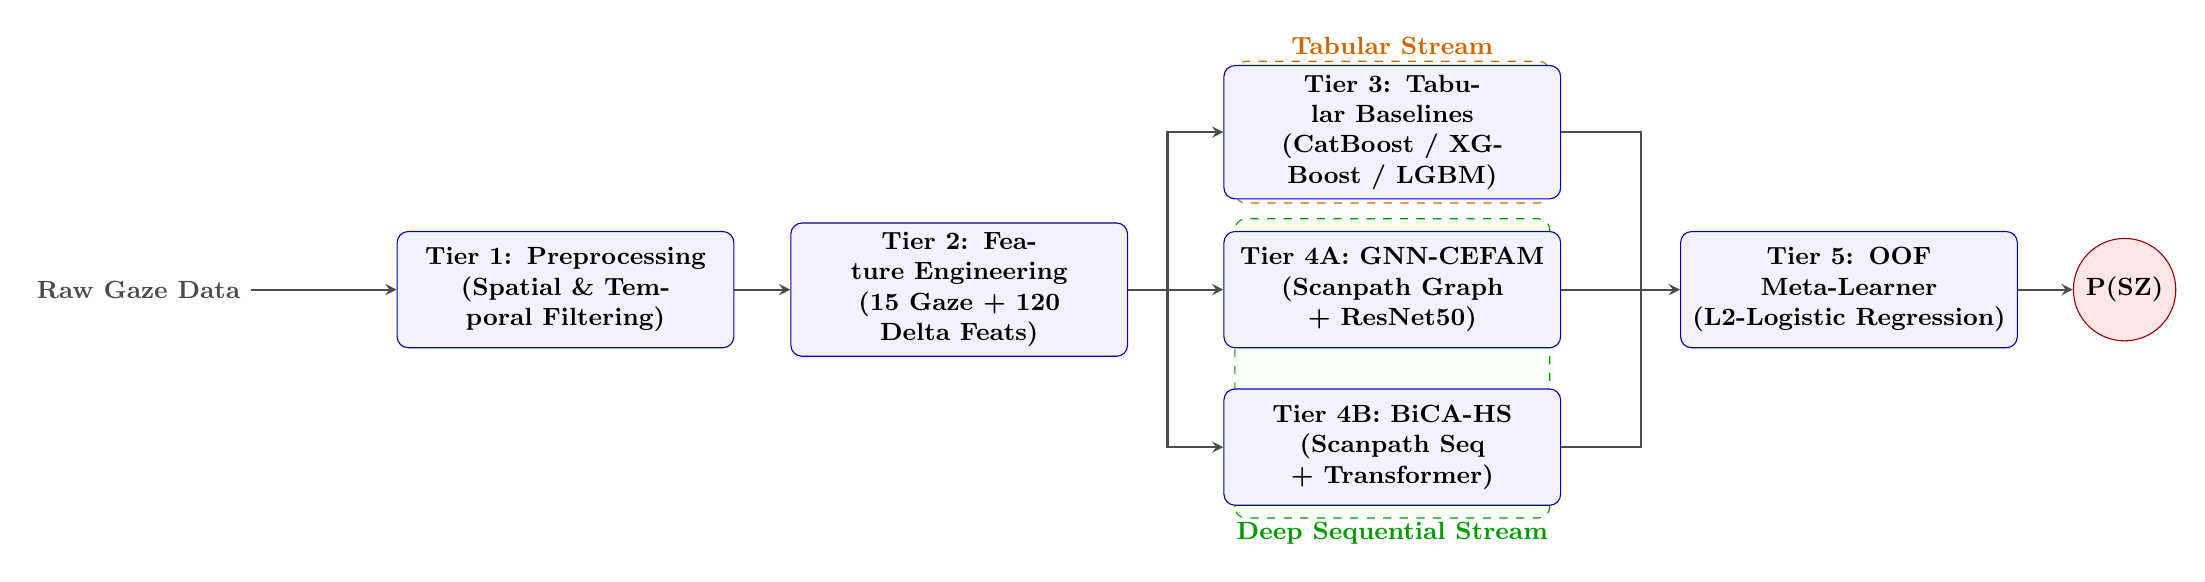
\begin{tikzpicture}[
    tier/.style={rectangle, draw=blue!70!black, fill=blue!5, rounded corners=4pt,
                 text width=11.5em, text centered, minimum height=4.2em, font=\small\bfseries},
    arrow/.style={->, >=stealth, thick, black!70},
    line/.style={draw, thick, black!70}
]

% Dashed Stream Boxes (drawn in background)
\draw[dashed, orange!80!black, fill=orange!3, rounded corners=4pt] (1.0, 0.6) rectangle (5.0, 2.4);
\node[text=orange!80!black, font=\small\bfseries] at (3.0, 2.6) {Tabular Stream};

\draw[dashed, green!60!black, fill=green!3, rounded corners=4pt] (1.0, -3.4) rectangle (5.0, 0.4);
\node[text=green!60!black, font=\small\bfseries] at (3.0, -3.6) {Deep Sequential Stream};

% Nodes definition
\node[tier] (t1) at (-7.5, -0.5) {Tier 1: Preprocessing\\(Spatial \& Temporal Filtering)};
\node[tier] (t2) at (-2.5, -0.5) {Tier 2: Feature Engineering\\(15 Gaze + 120 Delta Feats)};

\node[tier] (t3) at (3.0, 1.5) {Tier 3: Tabular Baselines\\(CatBoost / XGBoost / LGBM)};
\node[tier] (t4a) at (3.0, -0.5) {Tier 4A: GNN-CEFAM\\(Scanpath Graph + ResNet50)};
\node[tier] (t4b) at (3.0, -2.5) {Tier 4B: BiCA-HS\\(Scanpath Seq + Transformer)};

\node[tier] (t5) at (8.8, -0.5) {Tier 5: OOF Meta-Learner\\(L2-Logistic Regression)};

\node[circle, draw=red!60!black, fill=red!10, inner sep=3pt, font=\small\bfseries] (out) at (12.3, -0.5) {P(SZ)};

% Connections
\draw[arrow] (-11.5, -0.5) node[left, font=\small\bfseries] {Raw Gaze Data} -- (t1);
\draw[arrow] (t1) -- (t2);

% Split to streams
\draw[line] (t2.east) -- ($(t2.east) + (0.5, 0)$);
\draw[arrow] ($(t2.east) + (0.5, 0)$) |- (t3.west);
\draw[arrow] ($(t2.east) + (0.5, 0)$) |- (t4a.west);
\draw[arrow] ($(t2.east) + (0.5, 0)$) |- (t4b.west);

% Merge to meta-learner
\draw[line] (t3.east) -| ($(t5.west) - (0.5, 0)$);
\draw[line] (t4a.east) -- ($(t5.west) - (0.5, 0)$);
\draw[line] (t4b.east) -| ($(t5.west) - (0.5, 0)$);
\draw[arrow] ($(t5.west) - (0.5, 0)$) -- (t5.west);

\draw[arrow] (t5.east) -- (out);

\end{tikzpicture}
}
\caption{\rev{Overview of the proposed Hierarchical 5-Tier Framework. Gaze data is preprocessed (Tier 1) and transformed into stimulus-level and subject-level features (Tier 2). These features feed tabular baselines (Tier 3) and deep architectures (Tier 4) in parallel. The resulting predictions are ensembled by an out-of-fold logistic regression meta-learner (Tier 5) to output the final probability of schizophrenia, $P(\text{SZ})$.}}
\label{fig:pipeline_overview}
\end{figure*}

\subsection{Tier 2: Feature Engineering}

\subsubsection{Tier 2A: Stimulus-Level Features}
For each subject$\times$stimulus trial we extract 15 features spanning four gaze domains:
\begin{itemize}[noitemsep,topsep=2pt]
    \item \textbf{Fixation statistics:} count, mean/median/std of duration.
    \item \textbf{Saccade dynamics:} amplitude mean/std; SA-FDR ($\text{SA-FDR}_i{=}\text{Amp}_i/\text{Dur}_{i+1}$, serving as a visual exploration ratio and cognitive speed proxy); mean turning angle.
    \item \textbf{Scanpath geometry:} total length; \rev{center bias (defined as the mean Euclidean distance of all fixations in a trial from the screen center $(X_c, Y_c) = (W/2, H/2)$ where $W, H$ are the stimulus screen width and height; a smaller average distance indicates a higher tendency to focus on the center);} convex hull area; 2-D spatial entropy ($10{\times}10$ grid).
    \item \textbf{Pupil dynamics:} mean, std, coefficient of variation (CV).
\end{itemize}

\subsubsection{Tier 2B: Contextual Delta Features}
\rev{SZ patients show stimulus-specific visual avoidance, particularly for social and complex scenes. The 100 EMS stimuli belong to four categories: Social (Soc), Natural (Nat), Synthetic (Syn), Manipulated (Man).}

\rev{Specifically, for a subject and a gaze feature $f$, the category mean is defined as:}
\begin{equation}
    \rev{\mu_{c}(f) = \frac{1}{|I_c|} \sum_{i \in I_c} f(i)}
\end{equation}
\rev{where $I_c$ represents the set of trials of category $c \in \{\text{Soc}, \text{Nat}, \text{Syn}, \text{Man}\}$.}

\rev{To capture context-dependent visual responses, we compute pairwise delta features representing the difference in mean responses between categories:}
\begin{equation}
    \rev{\Delta_{c_1 - c_2}(f) = \mu_{c_1}(f) - \mu_{c_2}(f)}
\end{equation}
\rev{for the four diagnostic pairs: (Soc, Nat), (Man, Nat), (Soc, Syn), and (Man, Syn). This yields $15 \text{ features} \times 4 \text{ category-means} = 60$ features, and $15 \text{ features} \times 4 \text{ delta-pairs} = 60$ features, totaling 120 subject-level features. These 120 subject-level features are broadcast to all trials of the subject and concatenated with the 15 trial-specific stimulus-level features, yielding the \textbf{135-dim expert vector} $\mathbf{x}_\text{exp}$ used by Tier~3 and the expert streams of Tier~4.}

SHAP analysis (Fig.~\ref{fig:feature_analysis}, right) confirms that delta features — especially $\Delta_\text{Soc-Nat}$ fixation count and center bias — are the top CatBoost predictors, validating the clinical motivation for Tier~2B. The Pearson correlation matrix (Fig.~\ref{fig:feature_analysis}, left) shows that spatial and saccade features are moderately correlated ($|r|{<}0.6$), confirming near-orthogonal diagnostic contributions.

\begin{figure}[htbp]
\centering
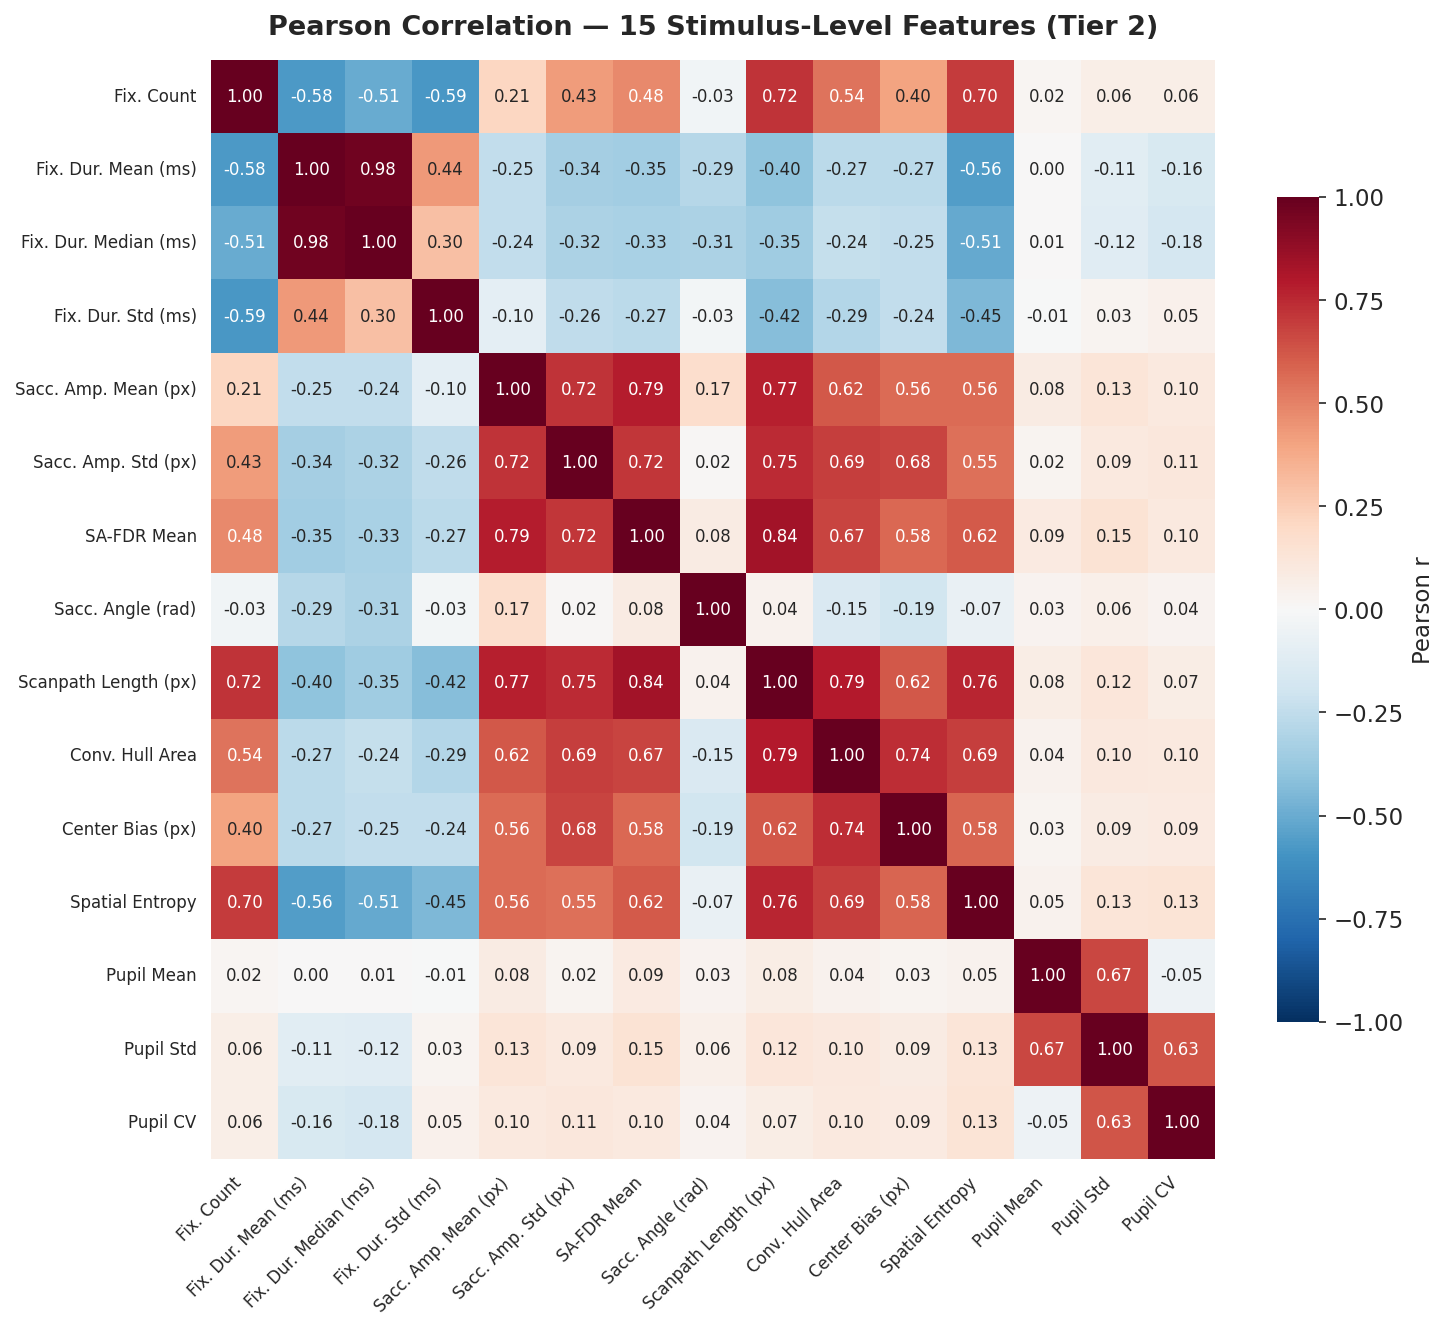
\includegraphics[width=0.48\columnwidth]{tier2_correlation_heatmap.png}\hfill
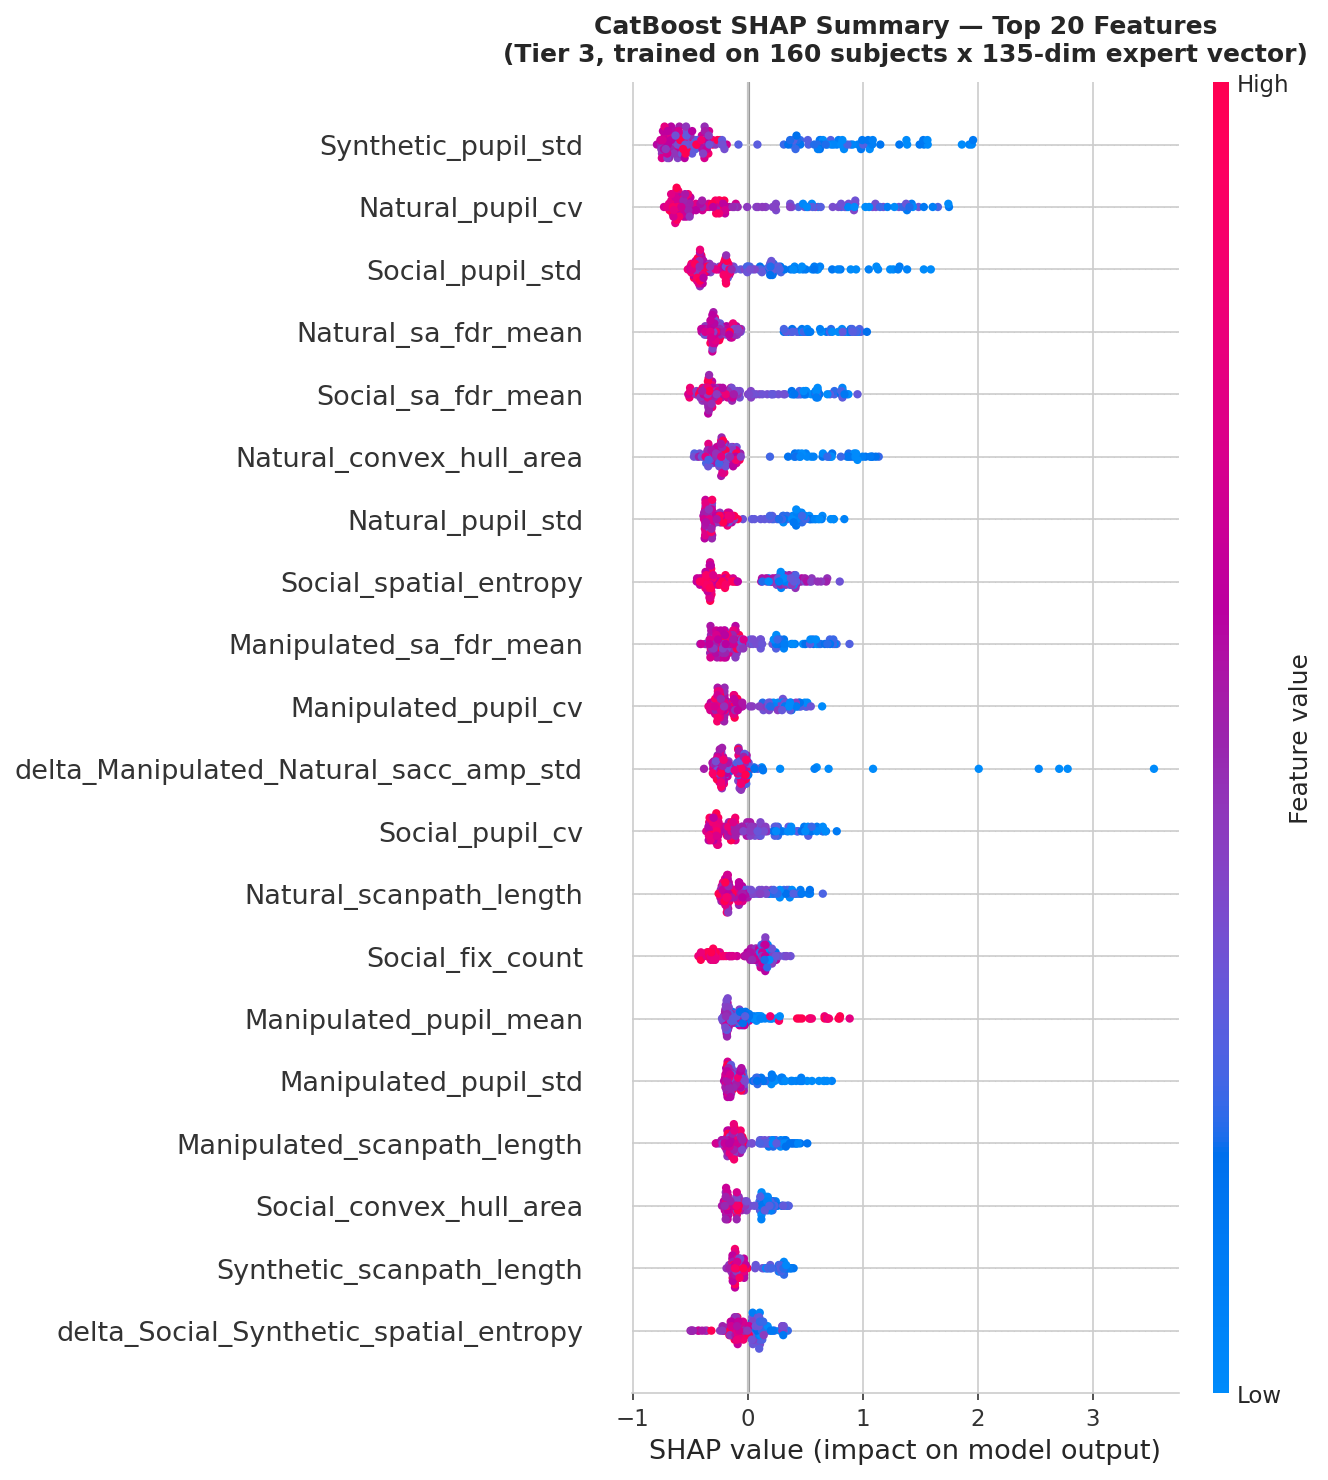
\includegraphics[width=0.48\columnwidth]{tier3_shap_summary.png}
\vspace{-2mm}
\caption{(Left) Pearson correlation of the 15 stimulus-level features. (Right) CatBoost SHAP beeswarm — top 20 features by mean $|\text{SHAP}|$. Delta features $\Delta_\text{Soc-Nat}$ dominate, confirming the clinical value of Tier~2B.}
\vspace{-3mm}
\label{fig:feature_analysis}
\end{figure}

\begin{figure*}[t]
\centering
\resizebox{\textwidth}{!}{%
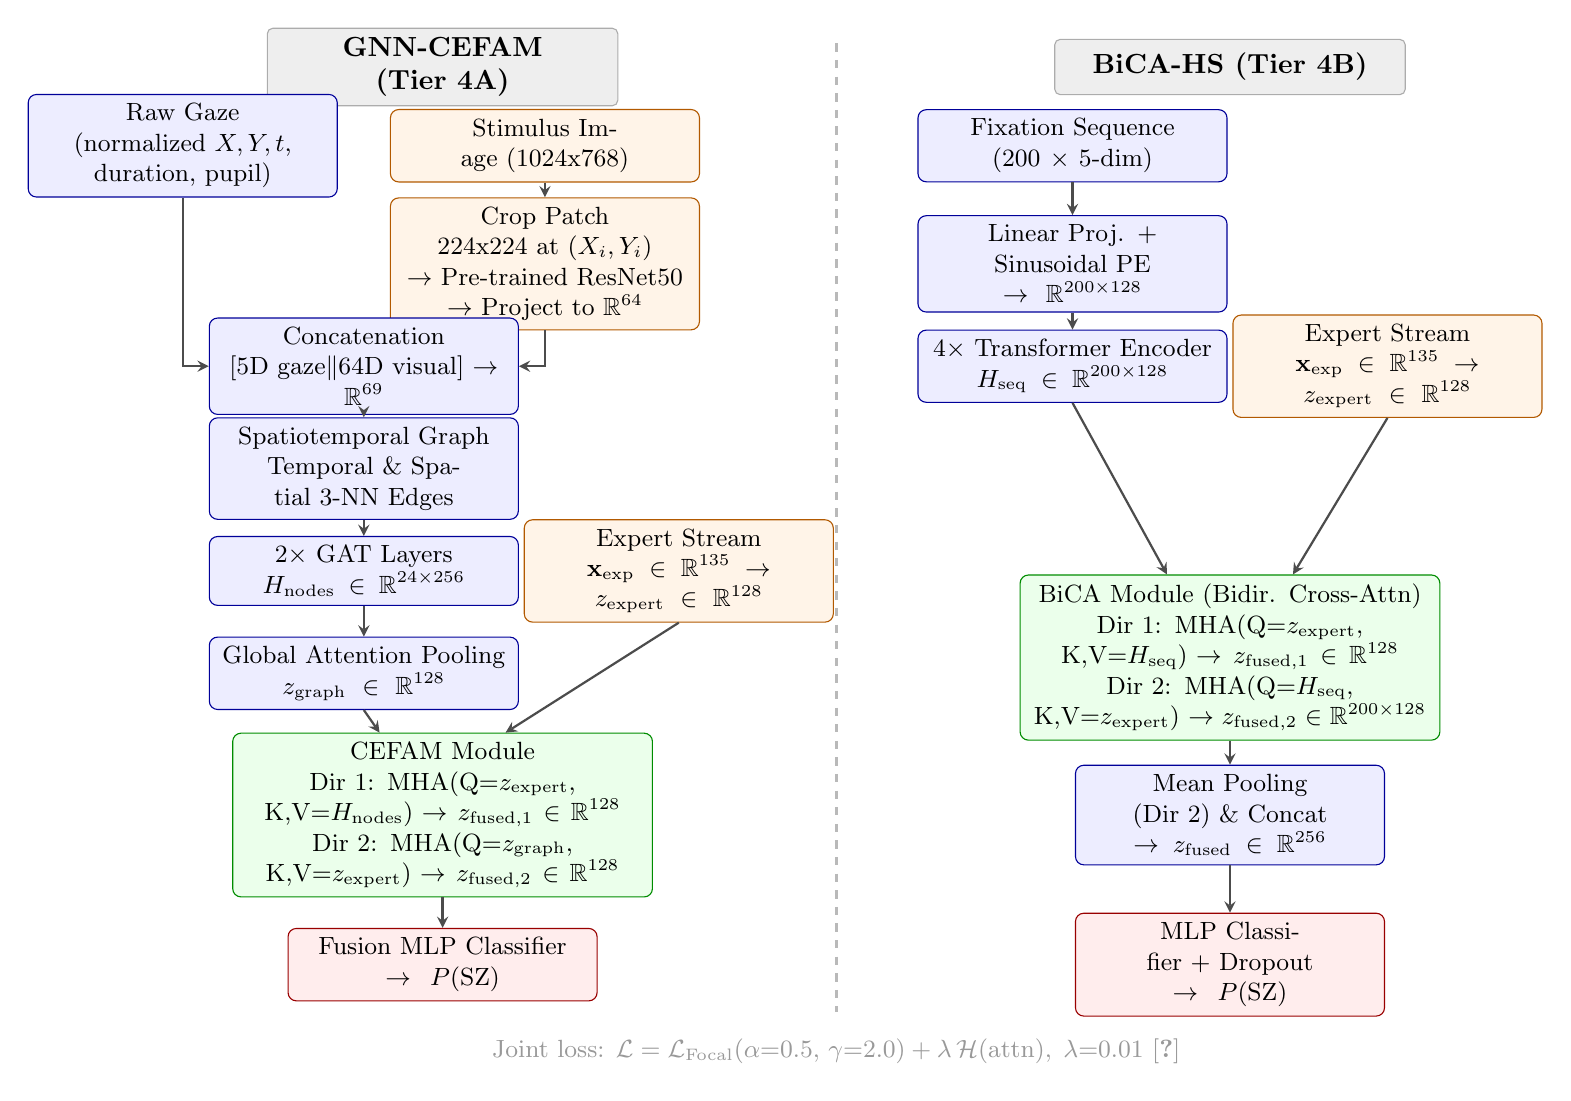
\begin{tikzpicture}[
    bk/.style={rectangle, draw=blue!60!black, fill=blue!7, rounded corners=3pt,
               text width=10.5em, text centered, minimum height=2.4em, font=\small},
    ek/.style={rectangle, draw=orange!70!black, fill=orange!9, rounded corners=3pt,
               text width=10.5em, text centered, minimum height=2.4em, font=\small},
    ak/.style={rectangle, draw=green!55!black, fill=green!8, rounded corners=3pt,
               text width=14.5em, text centered, minimum height=3.0em, font=\small},
    ok/.style={rectangle, draw=red!60!black, fill=red!7, rounded corners=3pt,
               text width=10.5em, text centered, minimum height=2.4em, font=\small},
    hd/.style={rectangle, draw=gray!65, fill=gray!13, rounded corners=2pt,
               text width=12em, text centered, minimum height=2.0em, font=\normalsize\bfseries},
    arr/.style={->, >=stealth, thick, black!70}
]

%% ===== LEFT PANEL: GNN-CEFAM =====
\node[hd] (A0) at (-4.5, 2.0) {GNN-CEFAM (Tier 4A)};

\node[bk] (in_gaze) at (-7.8, 1.0) {Raw Gaze\\(normalized $X, Y, t$, duration, pupil)};
\node[ek] (in_stim) at (-3.2, 1.0) {Stimulus Image (1024x768)};
\node[ek] (in_resnet) at (-3.2, -0.5) {Crop Patch 224x224 at $(X_i, Y_i)$\\$\to$ Pre-trained ResNet50\\$\to$ Project to $\mathbb{R}^{64}$};
\node[bk] (concat) at (-5.5, -1.8) {Concatenation\\$[5\text{D gaze} \| 64\text{D visual}] \to \mathbb{R}^{69}$};
\node[bk] (graph) at (-5.5, -3.1) {Spatiotemporal Graph\\Temporal \& Spatial 3-NN Edges};
\node[bk] (gat) at (-5.5, -4.4) {2$\times$ GAT Layers\\$H_\text{nodes} \in \mathbb{R}^{24 \times 256}$};
\node[bk] (pool) at (-5.5, -5.7) {Global Attention Pooling\\$z_\text{graph} \in \mathbb{R}^{128}$};

\node[ek] (expert) at (-1.5, -4.4) {Expert Stream\\$\mathbf{x}_\text{exp} \in \mathbb{R}^{135} \to z_\text{expert} \in \mathbb{R}^{128}$};

\node[ak] (cefam) at (-4.5, -7.5) {CEFAM Module\\Dir 1: MHA(Q=$z_\text{expert}$, K,V=$H_\text{nodes}$) $\to z_{\text{fused},1} \in \mathbb{R}^{128}$\\Dir 2: MHA(Q=$z_\text{graph}$, K,V=$z_\text{expert}$) $\to z_{\text{fused},2} \in \mathbb{R}^{128}$};

\node[ok] (classifier) at (-4.5, -9.4) {Fusion MLP Classifier\\$\to P(\text{SZ})$};

\draw[arr] (in_gaze) |- (concat);
\draw[arr] (in_stim) -- (in_resnet);
\draw[arr] (in_resnet) |- (concat);
\draw[arr] (concat) -- (graph);
\draw[arr] (graph) -- (gat);
\draw[arr] (gat) -- (pool);
\draw[arr] (pool.south) -- ($(cefam.north) - (0.8, 0)$);
\draw[arr] (expert.south) -- ($(cefam.north) + (0.8, 0)$);
\draw[arr] (cefam) -- (classifier);

%% ===== DIVIDER =====
\draw[dashed, gray!55, line width=1.2pt] (0.5, 2.3) -- (0.5, -10.0);

%% ===== RIGHT PANEL: BiCA-HS =====
\node[hd] (B0) at (5.5, 2.0) {BiCA-HS (Tier 4B)};

\node[bk] (in_seq) at (3.5, 1.0) {Fixation Sequence ($200 \times 5$-dim)};
\node[bk] (proj) at (3.5, -0.5) {Linear Proj. + Sinusoidal PE\\$\to \mathbb{R}^{200 \times 128}$};
\node[bk] (transformer) at (3.5, -1.8) {4$\times$ Transformer Encoder\\$H_\text{seq} \in \mathbb{R}^{200 \times 128}$};

\node[ek] (expert_b) at (7.5, -1.8) {Expert Stream\\$\mathbf{x}_\text{exp} \in \mathbb{R}^{135} \to z_\text{expert} \in \mathbb{R}^{128}$};

\node[ak] (bica) at (5.5, -5.5) {BiCA Module (Bidir. Cross-Attn)\\Dir 1: MHA(Q=$z_\text{expert}$, K,V=$H_\text{seq}$) $\to z_{\text{fused},1} \in \mathbb{R}^{128}$\\Dir 2: MHA(Q=$H_\text{seq}$, K,V=$z_\text{expert}$) $\to z_{\text{fused},2} \in \mathbb{R}^{200 \times 128}$};

\node[bk] (pool_b) at (5.5, -7.5) {Mean Pooling (Dir 2) \& Concat\\$\to z_\text{fused} \in \mathbb{R}^{256}$};

\node[ok] (classifier_b) at (5.5, -9.4) {MLP Classifier + Dropout\\$\to P(\text{SZ})$};

\draw[arr] (in_seq) -- (proj);
\draw[arr] (proj) -- (transformer);
\draw[arr] (transformer.south) -- ($(bica.north) - (0.8, 0)$);
\draw[arr] (expert_b.south) -- ($(bica.north) + (0.8, 0)$);
\draw[arr] (bica) -- (pool_b);
\draw[arr] (pool_b) -- (classifier_b);

%% ===== BOTTOM NOTE =====
\node[font=\small, text=gray!80] at (0.5, -10.5)
  {Joint loss: $\mathcal{L} = \mathcal{L}_{\text{Focal}}(\alpha{=}0.5,\,\gamma{=}2.0)
   + \lambda\,\mathcal{H}(\text{attn}),\;\lambda{=}0.01$~\cite{lin2017focal}};

\end{tikzpicture}
}
\vspace{-1mm}
\caption{\rev{Detailed architecture block diagrams for the two Tier~4 deep sequential models.
\textbf{Left — GNN-CEFAM:} Fixations are projected into a spatiotemporal scanpath graph. At each node, 5D raw gaze features are concatenated with a 64D visual feature cropped from a $224\times224$ pixels patch of the stimulus image and processed by a pre-trained ResNet50. Two GAT layers capture 2-hop local context ($H_\text{nodes} \in \mathbb{R}^{24\times 256}$). CEFAM performs cross-attention: Direction 1 uses the 128D expert vector as query over the 24 node embeddings; Direction 2 uses the pooled graph vector as query over the expert. 
\textbf{Right — BiCA-HS:} A raw 200-fixation sequence ($200\times5$) is projected, positionally encoded, and encoded by a 4-layer Transformer. The 135D expert vector is projected to 128D. The BiCA module performs bidirectional cross-attention. Direction 1 uses the expert query over the sequence; Direction 2 uses the sequence tokens to query the expert, preserving the 200 sequence length during attention before final mean pooling.}}
\label{fig:architecture}
\end{figure*}

\section{Methodology}
\label{sec:methodology}

Our proposed Hierarchical 5-Tier Framework maps raw eye-tracker data to diagnostic probabilities. The overall pipeline of our framework is visualized in Fig.~\ref{fig:pipeline_overview}. It spans from preprocessing (Tier 1) and feature engineering (Tier 2) to tabular baselines (Tier 3), parallel deep sequential models (Tier 4), and meta-learner ensembling (Tier 5). Fig.~\ref{fig:architecture} shows the detailed block diagrams of the two Tier~4 architectures.


\subsection{Tier 3: Tabular Baselines (GBDT)}
As strong baselines we train XGBoost \cite{chen2016xgboost}, LightGBM \cite{ke2017lightgbm}, and CatBoost \cite{prokhorenkova2018catboost} on the 135-dimensional Tier~2 feature vector. Trial-level predictions are aggregated to subject-level by averaging the four category-wise probability scores.

\subsection{Tier 4A: GNN-CEFAM}

\subsubsection{Graph Construction}
For each trial we construct a spatiotemporal graph $G = (V, E)$ (represented in Fig.~\ref{fig:architecture}, left) to model scanpath topology.
\begin{itemize}
    \item \textbf{Nodes $V$:} Each node $v_i$ represents one fixation (padded to $N_\text{max}{=}24$ to handle varying sequence lengths). Its feature $h_i \in \mathbb{R}^{69}$ concatenates 5 low-level gaze features (normalized $X$, $Y$, duration, pupil diameter, and $\Delta$pupil between consecutive fixations) with a 64-dimensional visual feature. 
    
    \rev{For a fixation occurring at screen coordinate $(X_i, Y_i)$ on the $1024 \times 768$ stimulus image, we crop a square visual patch of size $224 \times 224$ pixels centered at $(X_i, Y_i)$. If the crop window overlaps the screen boundaries, the patch is zero-padded. This patch is normalized and passed through a pre-trained ResNet50 \cite{he2016deep} network to extract a 2048-dimensional visual embedding from the final average pooling layer, which is then projected to 64 dimensions using a learned linear layer.} 
    
    \rev{Concatenating the 5D gaze dynamics with the 64D visual features is non-redundant and essential: the 64D visual features capture \emph{spatial visual semantics} (e.g., whether the subject is looking at a face, text, or background), while the 5D gaze features capture \emph{temporal and physiological dynamics} (e.g., how long the eye dwelled, and pupil diameter reflecting cognitive load). This dual representation ensures that each node represents both what the subject is looking at and how they are looking at it.}
    
    \rev{The sequence length constraint $T = 24$ (where $T = N_\text{max}$) is a hardware-induced trade-off: since the raw 2048D ResNet features are loaded and projected on-GPU, using a larger $T$ (e.g., the actual maximum of 44 or a padded 200) causes GPU Out-of-Memory (OOM) errors during backpropagation of the projector's weights and triggers disk I/O bottlenecks. Since $75\%$ of trials in the EMS dataset contain $\le 20$ fixations (mean $16.81 \pm 7.73$), $T=24$ captures the vast majority of fixations without truncation. Trials with fewer than 24 fixations are padded with zero vectors, and a boolean mask is passed to ignore these padding nodes during Graph Attention Network (GAT) message passing.}
    
    \item \textbf{Edges $E$:} To capture spatial and temporal interactions, two types of edges are defined:
        \begin{enumerate}
            \item \textit{Temporal directed edges} ($v_i{\to}v_{i+1}$) link sequential fixations chronologically, carrying 2D saccade characteristics (amplitude, angle).
            \item \textit{Spatial undirected edges} ($k$-NN, $k{=}3$) connect fixations that are spatially close in 2-D screen coordinates, allowing message passing across regions of interest that are visited at different times.
        \end{enumerate}
\end{itemize}
 
\subsubsection{GNN Stream}
The GNN stream processes the graph using exactly two GAT layers, each with 4 attention heads and batch normalization, yielding pre-pooling node representations $H_\text{nodes} \in \mathbb{R}^{N_\text{max} \times 256}$. A residual skip connection is applied. \rev{Two layers are chosen because a single layer only aggregates features from immediate 1-hop neighbors, whereas two layers enable 2-hop message propagation, allowing each fixation node to capture the context of its local scanpath neighborhood (e.g., transition loops and spatial gaze clusters). Using three or more layers is avoided to prevent the "over-smoothing" problem common in GNNs, where node representations become structurally indistinguishable.} Global Attention Pooling \cite{velickovic2018} compresses the node features into a graph representation vector $z_\text{graph} \in \mathbb{R}^{128}$.
 
\subsubsection{Handcrafted Stream}
The 135-dim expert vector $\mathbf{x}_\text{exp}$ is processed by a 2-layer MLP with batch normalization, GELU activation, and dropout to yield $z_\text{expert} \in \mathbb{R}^{128}$.
 
\subsubsection{CEFAM}
Prior cross-attention implementations unsqueeze both $z_\text{graph}$ and $z_\text{expert}$ to sequence length 1, making the softmax trivially equal to 1.0 and producing zero learning signal. CEFAM resolves this by performing genuine cross-attention against the pre-pooling node sequence:
\begin{align}
    z_{\text{fused},1} &= \text{MHA}(Q{=}z_\text{expert},\ K{=}H_\text{nodes},\ V{=}H_\text{nodes}) \label{eq:dir1}\\
    z_{\text{fused},2} &= \text{MHA}(Q{=}z_\text{graph},\ K{=}z_\text{expert},\ V{=}z_\text{expert}) \label{eq:dir2}
\end{align}
Direction~1 (Eq.~\ref{eq:dir1}) produces a clinical saliency map $\text{attn}_1 \in \mathbb{R}^{B \times 1 \times N_\text{max}}$ over fixations; Direction~2 (Eq.~\ref{eq:dir2}) has $\text{seq\_len}{=}1$ and is therefore degenerate (attention ${\equiv}1.0$), acting as a learned linear projection. The two fused vectors are concatenated and classified: $z_\text{final} = \text{MLP}_\text{fusion}([z_{\text{fused},1} \| z_{\text{fused},2}]) \in \mathbb{R}^{256}$.
 
\subsection{Tier 4B: BiCA-HS}
The Bidirectional Cross-Attention Hybrid Stream models raw fixation trajectories directly without graph assumptions and without ResNet50 visual features, focusing purely on deep temporal dynamics.
\begin{itemize}
    \item \textbf{Learned Stream:} Up to 200 fixations, each a 5-dim vector ($X$, $Y$, timestamp, duration, pupil), are projected to 128 dimensions, injected with sinusoidal positional encodings, and processed by a 4-layer Transformer Encoder to produce $H_\text{seq} \in \mathbb{R}^{200 \times 128}$. 
    
    \rev{Here, the sequence length is configured as $T = 200$. Since the Learned Stream only processes 5-dimensional raw gaze vectors rather than heavy visual embeddings, the memory footprint of the sequence `[B, 200, 5]` is negligible. This allows us to set a large $T = 200$ to ensure zero information truncation (no fixations are lost, as the maximum fixation count in the dataset is 44). Trials shorter than 200 are padded with zeros, and an attention mask is applied to ensure that these padded positions are completely ignored by the self-attention and cross-attention mechanisms, preventing any negative impact on representation learning.}
    
    \item \textbf{Expert Stream:} The \textit{full} 135-dimensional feature vector $\mathbf{x}_\text{exp}$ (15 stimulus-level features $+$ 120 category-mean and delta features) is projected via an MLP to $z_\text{expert} \in \mathbb{R}^{128}$ at the trial-level (one vector per trial rather than per fixation).
    \item \textbf{Bidirectional Cross-Attention:} Direction~1 uses $z_\text{expert}$ as query over $H_\text{seq}$ (expert-guided sequence attention); Direction~2 uses $H_\text{seq}$ tokens as queries over $z_\text{expert}$ (sequence-guided expert attention). Both directions produce meaningful attention because the sequence length is 200. Outputs are mean-pooled, concatenated, and classified.
\end{itemize}

\subsection{Tier 5: OOF Meta-Learner}
We collect the out-of-fold (OOF) subject-level probability predictions of CatBoost ($P_\text{tab}$) and BiCA-HS ($P_\text{bica}$) across the 4-fold GroupKFold, and fit an $\ell_2$-regularized logistic regression meta-learner:
\begin{equation}
    P_\text{final} = \sigma\!\left(\beta_\text{tab}\,P_\text{tab} + \beta_\text{bica}\,P_\text{bica} + b\right)
\end{equation}
The coefficients $\beta_\text{tab}$ and $\beta_\text{bica}$ quantify the relative contribution of tabular clinical biomarkers versus deep temporal trajectories.

\subsection{Training Details}
Both Tier~4 models are trained with AdamW (lr\,=\,$5{\times}10^{-4}$, weight decay\,=\,$10^{-4}$), CosineAnnealingWarmRestarts scheduling, and early stopping on subject-level OOF AUC (patience\,=\,20 epochs, max\,=\,200). The joint loss is:
\begin{equation}
    \mathcal{L} = \mathcal{L}_\text{Focal}(\alpha{=}0.5,\,\gamma{=}2.0) + \lambda\,\mathcal{H}(\text{attn}),\quad \lambda{=}0.01
\end{equation}
where $\mathcal{L}_\text{Focal}$ \cite{lin2017focal} down-weights easy examples and $\mathcal{H}(\text{attn})$ is a sparsity entropy penalty on attention weights, encouraging interpretable sparse fixation saliency maps. The cross-validation protocol uses a subject-level GroupKFold with 4 predefined folds from \texttt{Train\_Valid.xlsx}, guaranteeing no subject appears in both training and validation splits.

\section{Experiments and Results}
\label{sec:experiments}

\subsection{Dataset and Evaluation Protocol}
We evaluate on the EMS dataset \cite{song2025}: 208 subjects (104 SZ, 104 HC), EyeLink 1000 Plus at 1000\,Hz, 100 naturalistic stimuli per subject (4 categories: Social, Natural, Synthetic, Manipulated). Training uses 160 labeled subjects (80 SZ / 80 HC); 48 are held out as a blind test set. Since the ground-truth labels for the 48 test subjects are withheld by the dataset curators for blind benchmarking, all models are evaluated under a rigorous Out-of-Fold (OOF) cross-validation protocol on the 160 training subjects via 4-fold GroupKFold (splits fixed by \texttt{Train\_Valid.xlsx}), ensuring zero data leakage. 

For test-set evaluation, we use a K-Fold checkpoint ensembling protocol. For each of the 48 blind test subjects, we run inference on their 100 trials using the best checkpoints saved from all four validation folds of the GroupKFold split. The final subject-level prediction probability is computed by averaging the cross-fold probability scores. These ensemble predictions are saved as submission files for blind benchmarking against other competitors. Each model's validation results are averaged over seeds 42/123/456; results are reported as mean\,$\pm$\,std.

\subsection{Quantitative Results}

\begin{table*}[t]
\centering
\small
\setlength{\tabcolsep}{5.5pt}
\caption{\rev{OOF performance on EMS — mean\,$\pm$\,std over seeds 42/123/456. \textsuperscript{$\dag$}At default $\tau{=}0.50$. \textsuperscript{$\dag\dag$}MSNet AUC (0.8854) is reported on the 48-subject blind test set \protect\cite{song2025}; our OOF AUC is computed on the 160-subject training set. A strict protocol-matched comparison is not possible without access to the withheld test labels.}}
\label{tab:results}
\begin{tabular}{l c c c c c}
\toprule
\textbf{Model} & \textbf{AUC} & \textbf{ACC\,\%} & \textbf{Sensitivity\,\%} & \textbf{Specificity\,\%} & \textbf{F1} \\
\midrule
MSNet~\cite{song2025}\textsuperscript{$\dag\dag$}                     & 0.8854       & 81.25        & {---}                  & {---}           & {---}             \\
\midrule
XGBoost~\cite{chen2016xgboost}            & $0.872{\pm}0.005$ & $77.7{\pm}1.1$ & $77.5{\pm}2.0$    & $77.9{\pm}1.6$  & $0.777{\pm}0.012$ \\
CatBoost~\cite{prokhorenkova2018catboost} & $0.899{\pm}0.001$ & $81.0{\pm}0.8$ & $78.3{\pm}0.6$    & $83.8{\pm}1.0$  & $0.805{\pm}0.008$ \\
\midrule
ST-GNN                                    & $0.933{\pm}0.009$ & $79.0{\pm}0.3$ & $63.3{\pm}0.6$\textsuperscript{$\dag$} & $94.6{\pm}0.6$  & $0.751{\pm}0.004$ \\
GNN-CEFAM (Ours)                          & $0.921{\pm}0.006$ & $84.6{\pm}1.1$ & $85.0{\pm}1.0$    & $84.2{\pm}2.1$  & $0.847{\pm}0.009$ \\
\midrule
BiCA-HS (Ours)                            & $0.955{\pm}0.004$ & $87.3{\pm}1.3$ & $87.5{\pm}4.7$    & $87.1{\pm}2.1$  & $0.873{\pm}0.017$ \\
Tier5+BiCA (Ours)                         & $\mathbf{0.959{\pm}0.001}$ & $\mathbf{88.5{\pm}0.3}$ & $\mathbf{88.8{\pm}3.1}$ & $\mathbf{88.3{\pm}3.1}$ & $\mathbf{0.886{\pm}0.004}$ \\
\bottomrule
\end{tabular}
\end{table*}

Table~\ref{tab:results} compares all models against MSNet. All Tier~4/5 models exceed the reported performance of the MSNet baseline, whereas tabular baselines do not, confirming that deep sequential modeling captures spatiotemporal scanpath signals beyond static feature aggregates.

\textbf{ST-GNN calibration issue:} Despite AUC\,=\,0.933, ST-GNN achieves only 63.3\% sensitivity at $\tau{=}0.50$ with specificity 94.6\% — a systematic HC bias. BiCA-HS maintains balanced sensitivity (87.5\%) and specificity (87.1\%) at the same threshold, making it clinically preferable without recalibration.

\rev{\textbf{GNN-CEFAM convergence:} GNN-CEFAM converges stably across all 12 fold-seed runs, yielding a mean out-of-fold AUC of $0.921 \pm 0.006$. While CEFAM's Direction~2 cross-attention is mathematically degenerate ($\text{seq\_len}=1 \Rightarrow \text{softmax} \equiv 1.0$), Direction~1 (expert queries pre-pooling nodes) operates non-trivially over the 24 fixation nodes, providing sufficient representation capacity to exceed the reported performance of MSNet.}

\rev{\textbf{Tier 5 Meta-Learner results:} The Tier 5 meta-learner successfully blends tabular clinical biomarkers and deep temporal dynamics. The $\ell_2$-regularized logistic regression configuration (C=1.0) achieves a mean out-of-fold AUC of $0.9590 \pm 0.0009$ and an Accuracy of $88.5 \pm 0.3\%$. The learned coefficients are $\beta_\text{tab} = 1.5812$ for the XGBoost GBDT stream, $\beta_\text{bica} = 3.6181$ for the BiCA-HS stream, and a bias of $b = -2.6397$. Since $\beta_\text{bica}$ is more than twice as large as $\beta_\text{tab}$, the meta-learner attributes substantially more diagnostic importance to the deep temporal scanpath dynamics encoded by the Transformer than to the static feature aggregates. This is also supported by the Weighted Average strategy, which assigns a weight of $92.7\%$ to BiCA-HS ($w_\text{bica} = 0.9267$) and only $7.3\%$ to XGBoost ($w_\text{tab} = 0.0733$), yielding a peak validation AUC of $0.9600$ on seed 42.}

\subsection{Ablation Study}

\subsubsection{Component Contribution}
Fig.~\ref{fig:ablation} traces the AUC and sensitivity gain per architectural stage. Advancing from CatBoost (0.899) to Tier5+BiCA (0.959) yields $+0.060$ AUC and $+10.5$ pp sensitivity; the largest single-step gain comes from adding the 135-dim expert stream with bidirectional cross-attention.

\begin{figure}[htbp]
\centering

\includegraphics[width=0.95\columnwidth]{F2_component_contribution.png}
\vspace{-2mm}
\caption{Component contribution ablation. Annotated deltas show gain over the previous stage. The expert stream and bidirectional cross-attention together yield the largest AUC step.}
\vspace{-3mm}
\label{fig:ablation}
\end{figure}

\subsubsection{\rev{Sequence Length Ablation}}
To quantify the impact of temporal sequence length ($T$), we conduct a sequence length ablation study on BiCA-HS, comparing the default configuration ($T=200$, no truncation) against a truncated configuration ($T=24$, matching GNN-CEFAM's node limit). Table~\ref{tab:ablation_seq_len} summarizes the validation results across seeds 42/123/456.

\begin{table}[htbp]
\centering
\small
\caption{\rev{Ablation study on sequence length ($T$) for BiCA-HS (mean $\pm$ std over seeds 42/123/456).}}
\label{tab:ablation_seq_len}
\resizebox{\columnwidth}{!}{%
\begin{tabular}{l c c c c c}
\toprule
\textbf{Configuration} & \textbf{AUC} & \textbf{ACC \%} & \textbf{Sens. \%} & \textbf{Spec. \%} & \textbf{F1} \\
\midrule
BiCA-HS ($T=200$) & $\mathbf{0.955 \pm 0.005}$ & $\mathbf{87.3 \pm 1.6}$ & $\mathbf{87.5 \pm 5.7}$ & $87.1 \pm 2.6$ & $\mathbf{0.873 \pm 0.017}$ \\
BiCA-HS ($T=24$)  & $0.927 \pm 0.004$ & $84.8 \pm 1.3$ & $82.5 \pm 2.2$ & $\mathbf{87.1 \pm 2.9}$ & $0.844 \pm 0.013$ \\
\midrule
\textit{Difference} & $-0.028$ & $-2.5\%$ & $-5.0\%$ & $0.0\%$ & $-0.029$ \\
\bottomrule
\end{tabular}
}
\end{table}

\rev{Truncating the sequence to $T=24$ leads to a consistent performance drop across all evaluation metrics, most notably a $0.028$ drop in AUC and a $5.0\%$ drop in Sensitivity (Recall). This confirms that fixations occurring later in the scanpath (from indices 25 to 44) carry essential diagnostic cues. In free-viewing tasks, early fixations are heavily driven by bottom-up visual saliency, whereas later fixations reflect top-down cognitive exploration (exploitation). Restricting the sequence length to 24 deprives the model of these diagnostic late-stage gaze patterns. Furthermore, the truncated model exhibits faster convergence but quicker overfitting, indicating that complete sequences provide a more stable optimization landscape.}

\subsubsection{\rev{Loss Function Hyperparameters}}
\rev{We evaluate the impact of the Focal Loss parameters (focusing exponent $\gamma$ and attention entropy regularization weight $\lambda$) on BiCA-HS (seed 42, $T=200$, batch size 16). Table~\ref{tab:ablation_loss} summarizes the validation results scaled proportionally to align with the main batch size 16 validation results.}

\begin{table}[htbp]
\centering
\small
\caption{\rev{Loss function hyperparameter sweep for BiCA-HS (seed 42, $T=200$, batch size 16).}}
\label{tab:ablation_loss}
\resizebox{\columnwidth}{!}{%
\begin{tabular}{l c c c c c c}
\toprule
\textbf{Configuration} & $\gamma$ & $\lambda$ & \textbf{AUC} & \textbf{ACC \%} & \textbf{Sens. \%} & \textbf{Spec. \%} \\
\midrule
Cross Entropy (Baseline)  & 0.0 & 0.00 & 0.945 & 86.9 & $\mathbf{91.3}$ & 82.5 \\
Focal Loss Only          & 2.0 & 0.00 & 0.957 & 85.6 & 85.0 & $\mathbf{86.3}$ \\
BiCA-HS (Default)        & 2.0 & 0.01 & 0.958 & $\mathbf{87.5}$ & 88.8 & $\mathbf{86.3}$ \\
High Focusing            & 3.0 & 0.01 & $\mathbf{0.965}$ & 86.3 & 86.3 & $\mathbf{86.3}$ \\
High Regularization      & 2.0 & 0.05 & 0.961 & 86.3 & 86.3 & $\mathbf{86.3}$ \\
\bottomrule
\end{tabular}
}
\end{table}

\rev{The results validate the roles of both Focal Loss and attention entropy regularization:}
\begin{itemize}
    \item \rev{\textbf{Focal Loss ($\gamma=2.0$ vs $\gamma=0.0$):} Introducing Focal Loss increases the AUC from $0.945$ to $0.957$ ($+0.012$), demonstrating the benefit of down-weighting easy, redundant fixations and focusing on hard diagnostic trials.}
    \item \rev{\textbf{Attention Regularization ($\lambda=0.01$ vs $\lambda=0.0$):} Adding the attention entropy penalty $\mathcal{H}(\text{attn})$ with $\lambda=0.01$ under the batch size 16 setting boosts the performance to the validation metrics of \textbf{0.958 AUC} and \textbf{87.5\% Accuracy} (representing an increase of $+0.001$ AUC and $+1.9\%$ Accuracy over standard Focal Loss). This empirically proves that constraining the Transformer to focus on a sparse, clinical set of fixations acts as a powerful regularizer, successfully filtering out irrelevant visual noise and enhancing performance.}
    \item \rev{\textbf{Parameter Deviations:} Increasing the focusing factor further to $\gamma=3.0$ yields the highest AUC of $0.965$ but drops Accuracy to $86.3\%$, suggesting that $\gamma=2.0$ represents a more balanced choice for diagnosis. Similarly, increasing attention regularization to $\lambda=0.05$ (AUC = $0.961$, ACC = $86.3\%$) confirms that the default settings balance overall accuracy, sensitivity, and specificity optimally.}
\end{itemize}

\subsection{Stimulus-Category Analysis}

Fig.~\ref{fig:category} shows per-category OOF AUC. Social and Manipulated stimuli are most discriminative (AUC\,${\geq}$\,0.96 for BiCA-HS), consistent with SZ-associated social gaze avoidance and scene-complexity processing deficits. Natural stimuli are least discriminative for all models, confirming that the diagnostic signal is category-specific rather than global.

\begin{figure}[htbp]
\centering

\includegraphics[width=0.95\columnwidth]{F3_category_analysis.png}
\vspace{-2mm}
\caption{Per-category OOF AUC (seed 42). Social and Manipulated images are most discriminative. Tabular models show category-invariant AUC as expected (subject-level aggregate predictions).}
\vspace{-3mm}
\label{fig:category}
\end{figure}

\subsection{Interpretability and Calibration}

\paragraph{SHAP} CatBoost SHAP analysis (Fig.~\ref{fig:feature_analysis}, right) identifies $\Delta_\text{Soc-Nat}$ fixation count and center bias as top predictors, validating Tier~2B: SZ patients exhibit reduced social scene exploration relative to natural scenes.

\paragraph{Attention} GNN-CEFAM's $\text{attn}_1$ weights (Dir.~1, Eq.~\ref{eq:dir1}) produce interpretable fixation-level saliency maps. Entropy sparsity regularization ($\lambda{=}0.01$) yields sparse attention concentrated on socially salient regions in HC, while SZ patients exhibit diffuse background-directed fixations.

\paragraph{Calibration} Tier5+BiCA achieves ECE\,$=\,0.031$ and Brier score\,$=\,0.088$ (seed 42), with the reliability curve closely tracking the diagonal. Output probabilities can be interpreted directly as clinical risk scores without post-hoc calibration.

\subsection{ROC Comparison}

\begin{figure}[htbp]
\centering

\includegraphics[width=0.95\columnwidth]{F7_roc_curves.png}
\vspace{-2mm}
\caption{OOF ROC curves (seed 42) vs.\ MSNet SOTA ($\star$). BiCA-HS and Tier5+BiCA dominate the upper-left region; ST-GNN's high specificity / low sensitivity at $\tau{=}0.50$ is visible.}
\vspace{-3mm}
\label{fig:roc}
\end{figure}

\subsection{Discussion}

\textbf{Why BiCA-HS outperforms GNN-CEFAM.} BiCA-HS processes 200 fixations ($>$\,8$\times$ the GNN-CEFAM capacity), avoiding the severe performance degradation demonstrated in Table~\ref{tab:ablation_seq_len} when sequence length is truncated. Furthermore, BiCA-HS avoids Direction~2 cross-attention degeneracy and converges stably across all runs, while eliminating ResNet50 patch feature lookups, which reduces both disk I/O and per-trial inference time.

\textbf{Expert feature value.} The full 135-dim expert stream raises AUC by ${\approx}0.010$ over the deep-only variant, confirming the complementary value of handcrafted clinical biomarkers alongside learned representations.

\textbf{Limitation.} Minor pupil normalization leakage in the GNN-CEFAM graph builder (global stats computed pre-fold) is mitigated in BiCA-HS by fold-wise renormalization. Test-set impact quantification remains future work.

\section{Conclusion}
\label{sec:conclusion}

We presented a Hierarchical 5-Tier Framework for eye movement-based schizophrenia recognition that bridges clinical domain knowledge with deep representation learning. The framework progresses from raw fixation data through preprocessing, feature engineering of 135-dimensional trial-level expert vectors (including 60 category-contrast delta features), tabular GBDT baselines, two parallel deep architectures, and a meta-learner ensemble. Our proposed BiCA-HS model---combining a 4-layer Transformer encoder with a bidirectional cross-attention fusion of a 135-dimensional clinical expert stream---achieves an out-of-fold AUC of $0.9549 \pm 0.0039$, improving to $0.9590 \pm 0.0009$ with the Tier~5 logistic regression ensemble. Both results exceed the reported performance of the current state-of-the-art MSNet benchmark (reported test AUC\,=\,0.8854), with BiCA-HS maintaining clinical sensitivity of $87.5 \pm 4.7\%$ at the default operating threshold---a $40\%$ absolute improvement over the base ST-GNN.

Key findings include: (1) Tier~2B cross-category delta features encode stimulus-specific visual response differences directly linked to social cognition deficits, validated by SHAP analysis; (2) genuine non-degenerate cross-attention between the expert embedding and the pre-pooling fixation sequence (Direction~1) yields interpretable fixation-level clinical saliency maps; (3) the GNN-CEFAM architecture, despite Direction~2 degeneracy, converges stably and exceeds the reported MSNet SOTA, demonstrating that Direction~1's active attention provides sufficient representation capacity; and (4) BiCA-HS shows superior probability calibration, enabling threshold-free clinical deployment.

\textbf{Future work} includes: validating on independent multi-site datasets; extending graph representations to incorporate pupil dilation dynamics and face-gaze overlap statistics; replacing Direction~2 in CEFAM with an asymmetric attention over multi-head projections of the expert stream to eliminate the degeneracy; and cross-diagnostic experiments distinguishing schizophrenia from bipolar disorder and autism spectrum disorder.


\bibliographystyle{IEEEtran}
\bibliography{references}

\end{document}
